\documentclass[11pt,a4paper]{article}

\usepackage[utf8]{inputenc}
\usepackage{amsmath,amssymb}
\usepackage[margin=2.5cm]{geometry}
\usepackage{graphicx}
\usepackage{xcolor}
\usepackage{enumitem}
\usepackage[skins]{tcolorbox}
\usepackage[colorlinks=true,linkcolor=violet!70!black,urlcolor=violet!70!black]{hyperref}

\definecolor{accent}{HTML}{534AB7}

\newtcolorbox{callout}{
  enhanced, frame hidden, boxrule=0pt, sharp corners,
  colback=accent!6, borderline west={2.5pt}{0pt}{accent},
  left=10pt, right=8pt, top=5pt, bottom=5pt, before skip=8pt, after skip=8pt
}

\setlist[itemize]{itemsep=2pt, topsep=4pt}
\setlist[enumerate]{itemsep=2pt, topsep=4pt}
\setlength{\parindent}{0pt}
\setlength{\parskip}{6pt}

\newcommand{\norm}[1]{\left\lVert #1 \right\rVert}

\title{Topic 12 --- Norms}
\author{}
\date{}

\begin{document}

\maketitle
\vspace{-2.2em}

\begin{center}
  \textbf{Subject:} Linear Algebra for ML \quad|\quad
  \textbf{Status:} growing \quad|\quad
  \textbf{MOC:} Math
\end{center}

\hrule
\vspace{4pt}

\begin{abstract}
\noindent A vector norm maps a vector to a \textbf{scalar} that measures how ``big'' the vector is.
Different rules give different norms: $L^1$, $L^2$, $L^3$, $L^\infty$, and the general $L^p$.
\end{abstract}

% ------------------------------------------------------------
\section{Why Norms?}

Taking two vectors, one is $a = \begin{bmatrix} 3 \\ -4 \end{bmatrix}$ and the other one is
$b = \begin{bmatrix} 0 \\ 5 \end{bmatrix}$, but we want to know \textbf{which one is bigger}:

$\rightarrow$ here we use \textbf{norms} (vector norm).

\subsection{Vector Norm}

\begin{callout}
A vector norm gives us a way to \textbf{measure how ``big'' a vector is}.
\end{callout}

\begin{itemize}
  \item Maps a vector to a \textbf{scalar} based on a specific rule.
\end{itemize}

% ------------------------------------------------------------
\section{Rules}

\[
  \begin{bmatrix} a_1 \\ a_2 \\ \vdots \\ a_n \end{bmatrix}
  \xrightarrow[L^1\ \text{Norm}]{|a_1| + |a_2| + \dots + |a_n|}
  \norm{a}_1 \;\rightarrow\; \text{scalar}
\]

\[
  \begin{bmatrix} a_1 \\ a_2 \\ \vdots \\ a_n \end{bmatrix}
  \xrightarrow[L^2\ \text{Norm}]{\sqrt{a_1^2 + a_2^2 + \dots + a_n^2}}
  \norm{a}_2
\]

\[
  \begin{bmatrix} a_1 \\ a_2 \\ \vdots \\ a_n \end{bmatrix}
  \xrightarrow[L^3\ \text{Norm}]{\sqrt[3]{|a_1|^3 + |a_2|^3 + \dots + |a_n|^3}}
  \norm{a}_3
\]

Then we can use the scalars to measure how ``big'' vectors are.

% ------------------------------------------------------------
\section{$L^1$ Norm}

\begin{callout}
\textbf{Adds up the absolute values} of a vector's components.
\end{callout}

\[
  \norm{a}_1 = 3 + |{-4}| = 7
\]

\[
  \norm{b}_1 = 0 + 5 = 5
\]

\[
  \norm{a}_1 > \norm{b}_1
\]

$\rightarrow$ So according to the $L^1$ norm, the first vector $a$ is \textbf{larger}.

\begin{itemize}
  \item Its contours are \textbf{diamonds}.
\end{itemize}

% ------------------------------------------------------------
\section{$L^2$ Norm}

\begin{callout}
Comes from the \textbf{Pythagorean theorem}.
\end{callout}

\begin{itemize}
  \item \textbf{Square} each component, \textbf{add} them up, and take the \textbf{square root}.
\end{itemize}

\[
  \norm{a}_2 = \sqrt{3^2 + (-4)^2} = 5
\]

\[
  \norm{b}_2 = \sqrt{0^2 + 5^2} = 5
\]

\[
  \norm{a}_2 = \norm{b}_2
\]

\begin{itemize}
  \item Its contours are \textbf{perfect circles}.
\end{itemize}

% ------------------------------------------------------------
\section{$L^3$ Norm}

\[
  \norm{a}_3 = \sqrt[3]{|a_1|^3 + |a_2|^3 + \dots + |a_n|^3}
\]

% ------------------------------------------------------------
\section{$L^\infty$ Norm}

\[
  \norm{a}_\infty = \max\{|x_1|, |x_2|\}
\]

\[
  a = \begin{bmatrix} 3 \\ -4 \end{bmatrix} \;\Rightarrow\;
  \norm{a}_\infty = \max\{3, |{-4}|\} = 4
\]

\[
  b = \begin{bmatrix} 0 \\ 5 \end{bmatrix} \;\Rightarrow\;
  \norm{b}_\infty = \max\{0, 5\} = 5
\]

% ------------------------------------------------------------
\section{$L^p$ Norm}

\[
  \begin{bmatrix} a_1 \\ a_2 \\ \vdots \\ a_n \end{bmatrix}
  \;\longrightarrow\;
  \left( |a_1|^p + |a_2|^p + \dots + |a_n|^p \right)^{1/p} = \norm{a}_p
\]

\begin{callout}
\textbf{Increase $p$} to get the \textbf{square} ($\square$) shape.
\end{callout}

% ------------------------------------------------------------
\section{Geometric View}

\begin{figure}[ht]
  \centering
  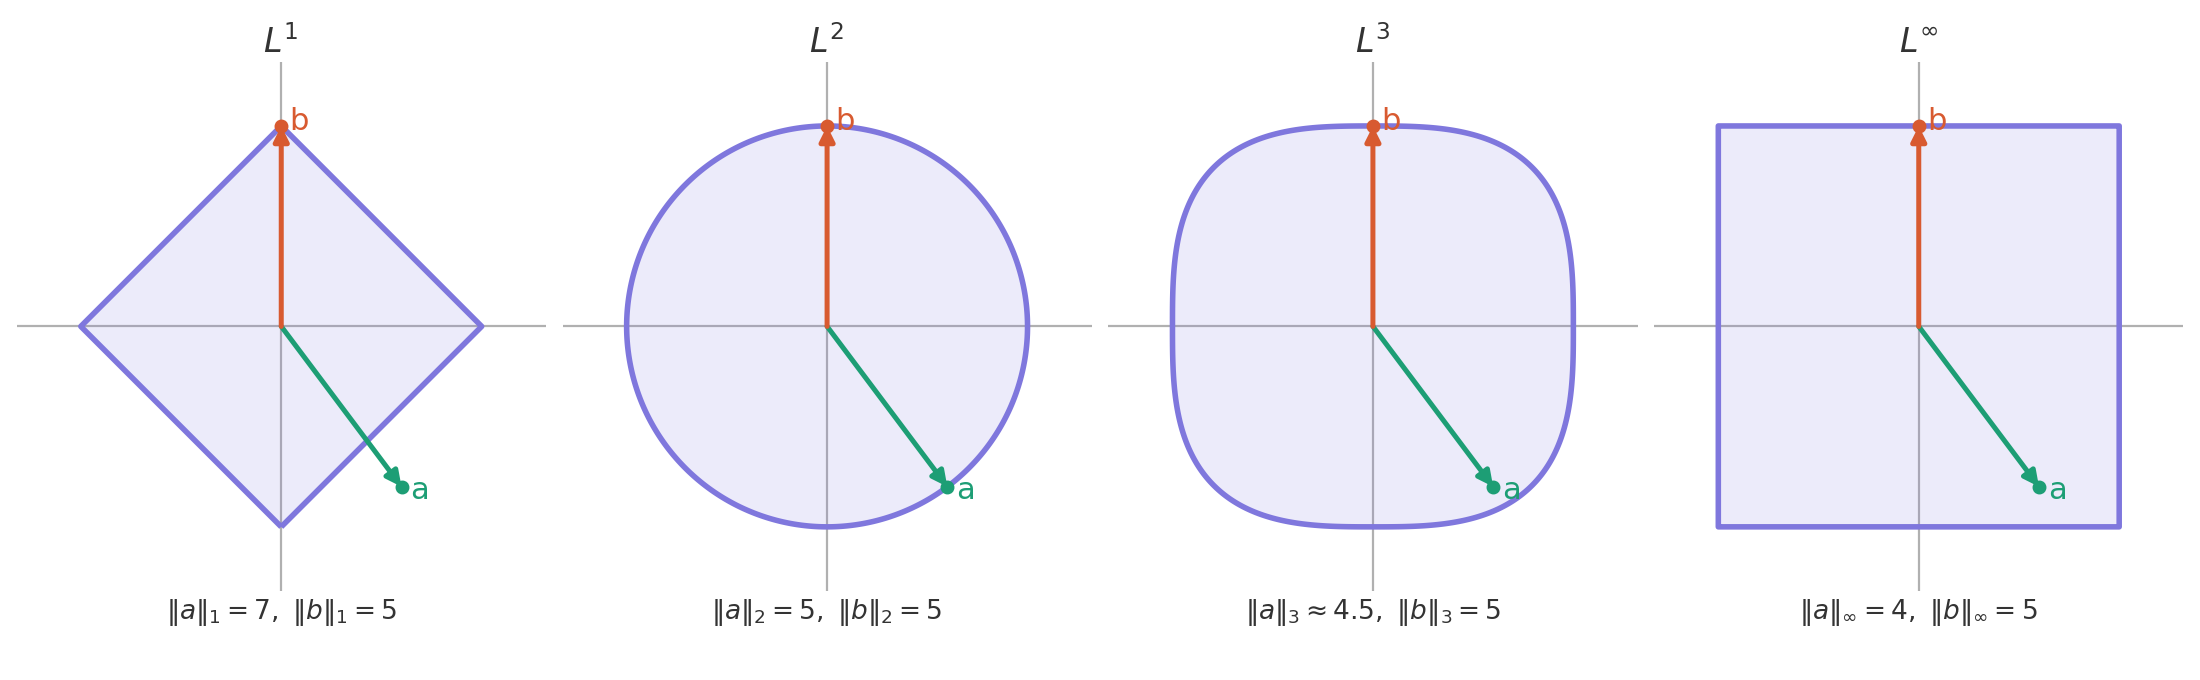
\includegraphics[width=\linewidth]{norm-contours.png}
  \caption{Each shape is the set of all vectors with norm $5$, for
  $a = (3,-4)$ and $b = (0,5)$. Inside the shape the norm is smaller than $5$,
  outside it is bigger.}
\end{figure}

\begin{itemize}
  \item $p = 1$ $\rightarrow$ diamond, $p = 2$ $\rightarrow$ circle, $p \to \infty$ $\rightarrow$ square.
  \item $a$ is bigger than $b$ under $L^1$, equal under $L^2$, and smaller under $L^3$ and $L^\infty$.
\end{itemize}

% ------------------------------------------------------------
\section*{Related Topics}

\begin{itemize}
  \item Topic 11 --- SVD
  \item Topic 02 --- Matrices
\end{itemize}

\vspace{6pt}
\hrule
\vspace{6pt}

\textit{Tags: \#linear-algebra \#norms \#vector-norm \#math \#phase-1}

\end{document}